\providecommand{\main}{../../..}

\documentclass[\main/main.tex]{subfiles}

\begin{document}

\chaptermark{Bouffard et al, Developmental biology, 2018}
\chapter{Article 1 : La
Fibrillarine est essentielle pour la progression de la phase S et la différenciation neuronale dans la rétine et la partie dorsale du mésencéphale du \pz{}
}

\section{Présentation de l'article 1}

\label{sec:bouffard}

% Introduction à la biogénèse des ribosomes et à Fbl
%
La biogénèse des ribosomes est un processus central pour les cellules qui recouvre l'ensemble des processus biologiques de production de ribosomes.
%
Elle implique un grand nombre de protéines telles que la Fibrillarine (Fbl) par exemple.
%
Cette protéine est aussi impliquée dans la méthylation des ARNs ribosomaux et des histones de l'ADN ribosomique.

% Effet notable de Fbl dans le vivant
%
Les études de la perte de fonction de gène Fbl chez la levure et la souris ont montré que
cette protéine était nécessaire à la survie cellulaire et au développement précoce.
%
De plus, il a été démontré que cette protéine joue un rôle important dans l'homéostasie cellulaire et l'identité des cellules souches.
%
Enfin, une surabondance de Fbl est mesurable chez les patients atteints de plusieurs formes de cancers, comme certains cancers du sein, certaines néoplasies prostatiques intra-épithéliales ou encore certains carcinomes des cellules squameuses cervicales.
%
Ainsi, la compréhension des mécanismes impliquant Fbl dans la régulationsdu cycle cellulaire pourrait ouvrir de nouvelles pistes dans des domaines thérapeutiques variés.

% Pourquoi utiliser le pz?
%
Le \pz{} a été choisi dans le cadre de cette étude car,
en plus des avantages présentés au chapitre~\ref{chap:zebra},
il possède une région ayant une croissance orientée dans la partie dorsale du cerveau moyen, le toit optique.
%
Cette région présente ainsi une colonne ordonnée de cellules possédant
un gradient de différenciation allant de la périphérie vers le centre de la structure.
%
L'observation de cette région est ainsi idéale pour étudier le rôle de la Fbl
dans le contrôle du cycle cellulaire et l'homéostasie cellulaire.
%

% Mesure du volume cérébral
%
Entre autre, deux marqueurs du système nerveux central ont été employés.
%
Le premier est un marqueur des lipides, le DiI, permettant de mesurer le volume de la matière blanche et des yeux.
%
Le second est un marquage par anticorps anti-HuC/D, protéine produite par le gène \textit{elavl3}.
%
Cette protéine étant impliquée dans la neurogénèse, son marquage permet de visualiser les corps cellulaires des neurones en différenciation.
%
En couplant ces deux marqueurs, il devient alors possible de mesurer la taille du cerveau, ainsi que de mesurer une anomalie de la neurogénèse.

% Résultat obtenus par la mesure du volume cérébral
%
Nous avons ainsi mis en évidence que les mutants \textit{fbl\textsuperscript{hi2581Tg}}
présentent une forte diminution du volume cérébral et du volume des yeux.
%
La réduction du volume cérébral est particulièrement notable
dans la partie dorsale du mésencéphale.
%
De plus, l'étude du marquage anti-HuC/D a permis de mettre en évidence
un défaut de neurogénèse dans ce même mésencéphale.

%Résumé des résultats
%
Dans le cadre de cette thèse, les résultats d'intérêts publiés au sein de
\emph{Developmental Biology}~\citep{bouffard_2018} sont les suivants:

\begin{itemize}
    
    \item
    L'emploi d'un marqueur des lipides permet de mesurer le volume de la matière blanche
    ainsi que le volume de la rétine.
    
    \item
    La mesure de ces deux volumes permet de mettre en évidence la présence d'une microcéphalie
    et d'une microphtalmie chez les mutants présentant une inhibition de la production de Fbl.
    
    \item
    Un marquage par un anticorps anti-HuC/D permet de détecter la matière grise.
    
    \item
    Une segmentation de la matière grise permet de mettre en évidence
    un défaut de neurogénèse au sein de la partie dorsale du mésencéphale de ces mutants.
    
    \item
    Ces deux marqueurs sont donc des candidats privilégiés
    dans l'analyse des volumes cérébraux.
    
    \item
    La segmentation de ces deux marqueurs permet ainsi de mettre en évidence
    de potentiel défauts induits par une mutation.
    
\end{itemize}


%% Mesure par segmentation manuelle
%
Pour réaliser ces mesures, nous avons réalisé des segmentations manuelles.
%
Dix-huit échantillons ont été segmentés,
six mutants homozygotes, six mutants hétérozygotes et six sauvages.
%
Pour cette étude, quatre segmentations ont été réalisées pour chaque échantillon:
Le cerveau, la zone HuC/D positive, l'oeil gauche et l'oeil droit.
%
Une semaine complète a été nécessaire pour réaliser les soixante-douze segmentations nécessaires.
%
La segmentation manuelle d'un grand nombre d'échantillons
nécessiterait donc l'emploi d'une personne uniquement dédiée à cette tâche.
%
Il est ainsi apparu nécessaire de mettre en place des algorithmes de segmentations automatiques
pour permettre le développement d'une plateforme d'HTA (analyse d'image à haut-débit) dédiée à l'étude
des défauts pouvant être provoqués par une mutation ou un produit neurotoxique.
%
Le développement de tels algorithmes a donc été un élément central de cette thèse, et est présenté en \autoref{sec:lempereur_info} et en \autoref{sec:HuC}.

De plus, cet étude met en évidence que la localisation d'un défaut de neurogénèse au sein de la partie dorsale du
mésencéphale n'aurait pas été possible par une image dorsale unique de l'échantillon.
%
La multiplication des plans d'acquisition  afin d'obtenir des voxels isotropiques devient ainsi une nécessité
pour permettre la mesure précise de déformation du système nerveux central.

\section{Article 1 publié dans Developmental Biology}

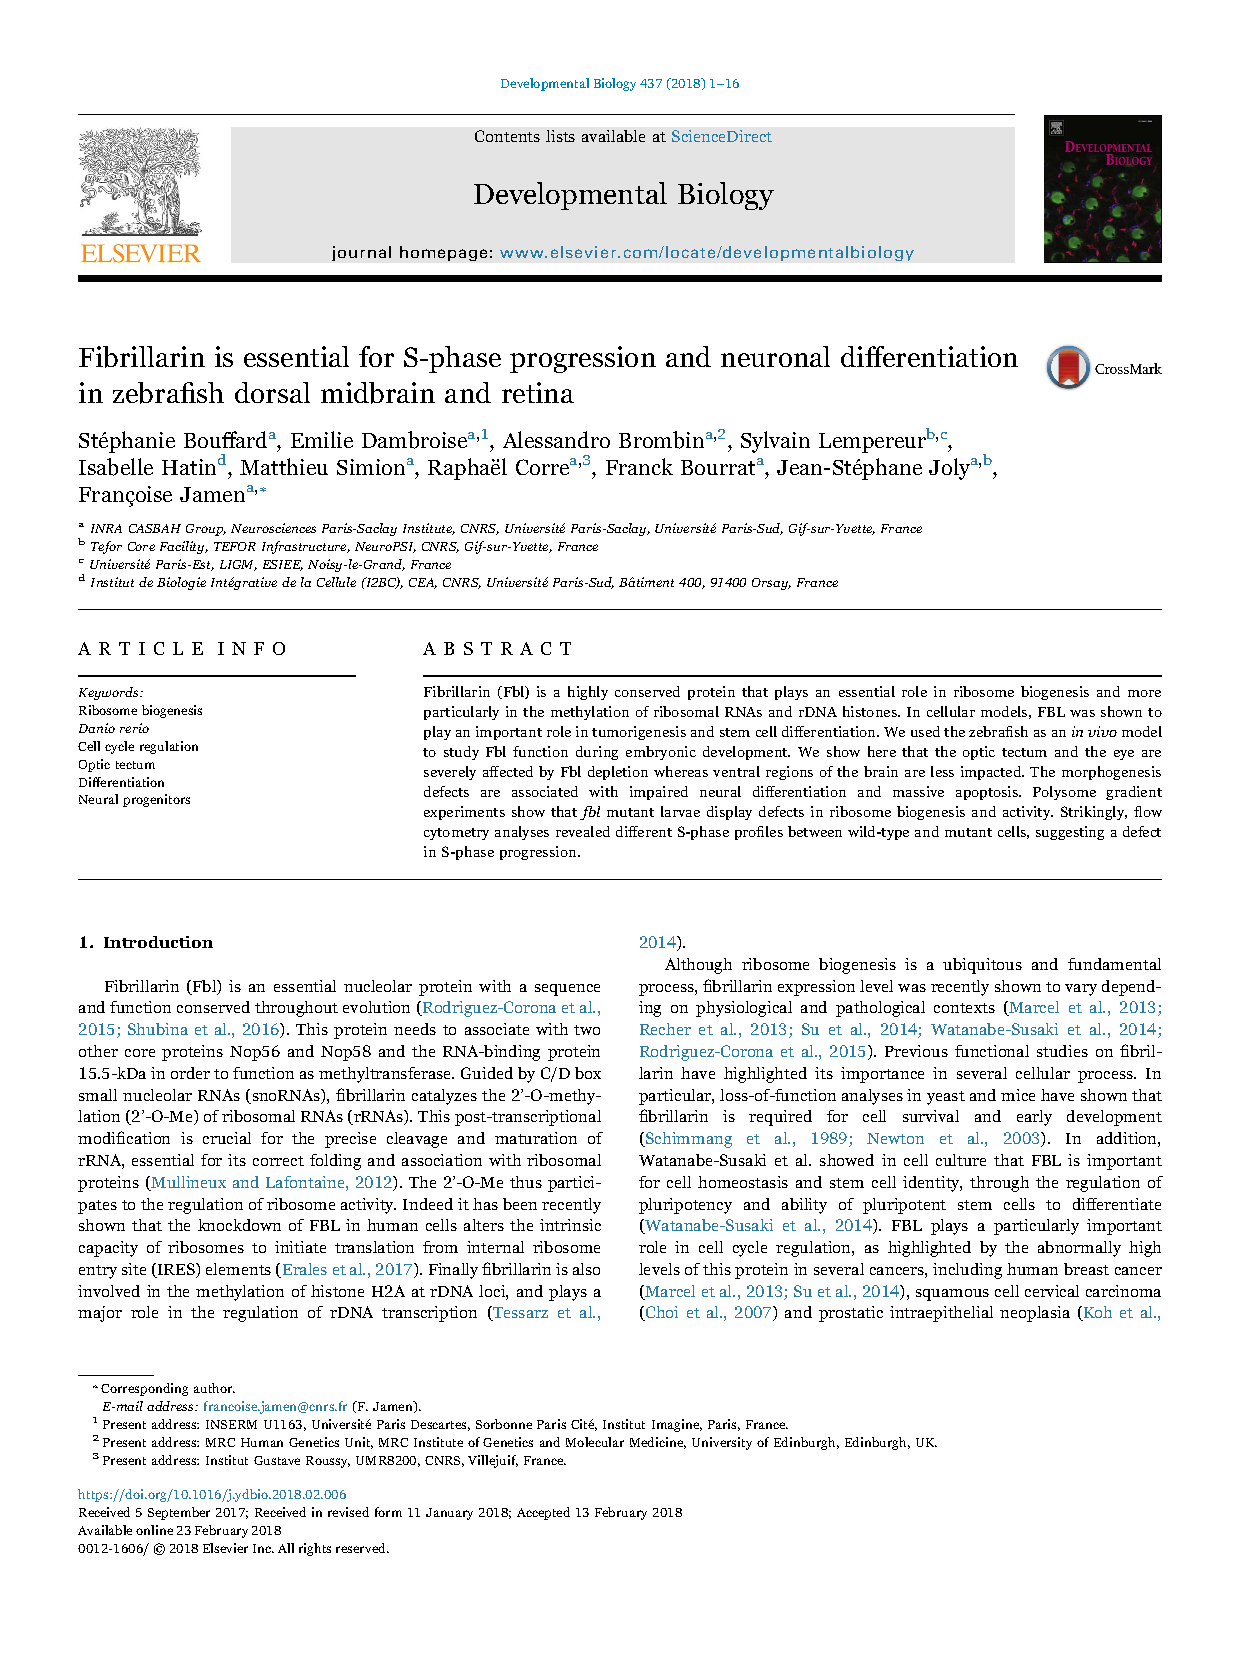
\includepdf[pages=-]{bouffard.pdf}

\end{document}
